\documentclass[11pt]{article}
\usepackage[parfill]{parskip}
\usepackage{graphicx}
\usepackage{wrapfig}
\usepackage{subcaption}
\usepackage[top=1in, bottom=1in, left=1in, right=1in]{geometry}
\bibliographystyle{plain}
\usepackage{amsmath}
\usepackage{amsfonts}
\usepackage{hyperref}
\usepackage{listings}
\usepackage{xcolor}
%%%%%%%%%%%%%%%%%%%%%%%%%%%%%%%%%%%%%%%%%%%%%%%%%%%%%%%%%%%%%%%
\usepackage{fancyhdr}
\pagestyle{fancy}
%%% Please add the author's last names
\lhead{Galois TA2 AMIDOL}
\rhead{ASKE Milestone 6 Report}
%%% Please use \cfoot{} to remove page numbers
\cfoot{ }
\renewcommand{\headrulewidth}{0pt}
\renewcommand{\footrulewidth}{0pt}
%%%%%%%%%%%%%%%%%%%%%%%%%%%%%%%%%%%%%%%%%%%%%%%%%%%%%%%%%%%%%%&
\usepackage{titlesec}
\titlespacing{\section}{0pt}{\parskip}{-.5\parskip}
\titlespacing{\subsection}{0pt}{\parskip}{- .5\parskip}
\titlespacing{\subsubsection}{0pt}{\parskip}{- .5\parskip}
\newcommand{\closeup}{\setlength{\itemsep}{-4pt}}

\colorlet{punct}{red!60!black}
\definecolor{background}{HTML}{EEEEEE}
\definecolor{delim}{RGB}{20,105,176}
\colorlet{numb}{magenta!60!black}

\usepackage{amsthm}

\newtheorem{mydef}{Definition}

\lstdefinelanguage{json}{
    basicstyle=\normalfont\ttfamily,
    numbers=left,
    numberstyle=\scriptsize,
    stepnumber=1,
    numbersep=8pt,
    showstringspaces=false,
    breaklines=true,
    frame=lines,
    backgroundcolor=\color{background},
    literate=
     *{0}{{{\color{numb}0}}}{1}
      {1}{{{\color{numb}1}}}{1}
      {2}{{{\color{numb}2}}}{1}
      {3}{{{\color{numb}3}}}{1}
      {4}{{{\color{numb}4}}}{1}
      {5}{{{\color{numb}5}}}{1}
      {6}{{{\color{numb}6}}}{1}
      {7}{{{\color{numb}7}}}{1}
      {8}{{{\color{numb}8}}}{1}
      {9}{{{\color{numb}9}}}{1}
      {:}{{{\color{punct}{:}}}}{1}
      {,}{{{\color{punct}{,}}}}{1}
      {\{}{{{\color{delim}{\{}}}}{1}
      {\}}{{{\color{delim}{\}}}}}{1}
      {[}{{{\color{delim}{[}}}}{1}
      {]}{{{\color{delim}{]}}}}{1},
}

\newcommand{\amidol}{\textsc{AMIDOL}}

\def\signed #1{{\leavevmode\unskip\nobreak\hfil\penalty50\hskip2em
  \hbox{}\nobreak\hfil(#1)%
  \parfillskip=0pt \finalhyphendemerits=0 \endgraf}}

\newsavebox\mybox
\newenvironment{aquote}[1]
  {\savebox\mybox{#1}\begin{quote}}
  {\signed{\usebox\mybox}\end{quote}}

\date{\vspace{-5ex}}
% Use this to get rid of the date

\usepackage{authblk}
\author[1]{Eric Davis}
\author[1]{Alec Theriault}
\author[1]{Ryan Wright}
\affil[1]{Galois, Inc}

%\setcounter{page}{0}



\title{May ASKE Milestone 6 Report for \amidol{}}

\begin{document}
\maketitle
\vspace{10pt}

\section{Introduction}

In this report we address the metamodeling process captured by
\amidol{}'s current implementation, discuss its relation to the
modeling stack proposed by the recent ASKE Phase II PI meeting, and a
present a roadmap for the future for \amidol{}, it's relation to the
ASKE program goals, and potential for collaboration with other
performers and the broader community.

\section{The Metamodeling Process}

The ASKE program is attempting to formalize the crucial components
required for machine-assisted modeling of complex systems, and the
machine-assisted extraction of knowledge from those models.  A large
portion of this effort, therefor, depends on the metamodeling
procedures used, and the assumptions about the abstractions and
representations of this process.  This process is captured in the
modeling stack, as shown in Figure \ref{Fig:Stack1}.

\begin{figure}
  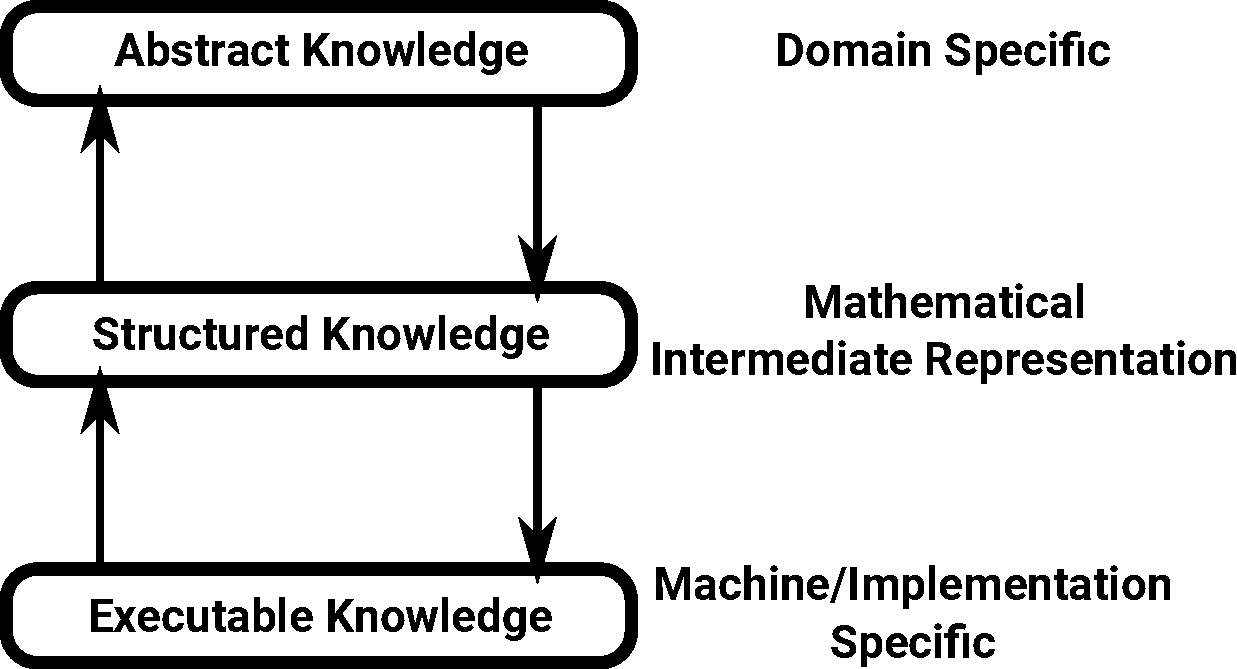
\includegraphics[width=\textwidth]{figs/stack-diagram-1.pdf}
  \caption{The ASKE modeling stack}
  \label{Fig:Stack1}
\end{figure}

The modeling stack consists of three discrete stages separated by the
way information is represented in each layer:

\begin{itemize}
\item \textbf{The Abtract Knowledge Layer}
\item \textbf{The Structured Knowledge Layer}
\item \textbf{The Executable Knowledge Layer}
\end{itemize}

As suggested by the names of these different layers, the primary
distinguishing characteristic of each layer is the way knowledge is
represented, the important characteristics of knowledge at that layer,
where interaction is concerned, and the goals of each layer.  The
Abstract Knowledge Layer primarily concerns itself with modeling
domain knowledge and assumptions.  It attempts to capture operational
and process semantics in a way which has meaning to domain scientists
and experts.  The Structured Knowledge Layer focuses on the syntactic
consequences of semantic domain knowledge from the Abstract Knowledge
Layer, and the Executable Knowledge Layer translates those syntactic
representations into executable machine code.

\begin{figure}
  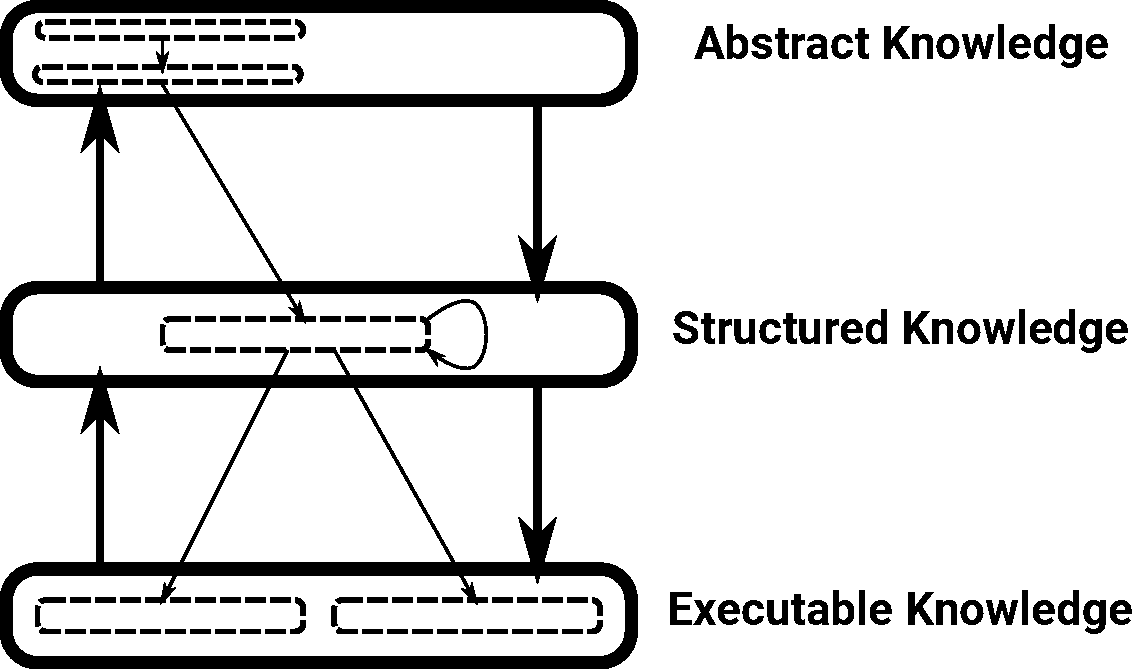
\includegraphics[width=\textwidth]{figs/stack-diagram-2.pdf}
  \caption{A complex view of the modeling stack composed of multiple
    applications in a given layer.}
  \label{Fig:Stack2}
\end{figure}

While the hierarchy presented for the layers in Figure
\ref{Fig:Stack1} represent the logical division of information and
representation in the modeling stack the result is not always a
simple stack composed of three applications, one at each layer.  We
envision the modeling stack as more of an abstraction that dictates
properties of the representational language of models at each layer of
the stack.  Multiple applications and implementations might exist in
each layer, sometimes coordinating and cooperating with other
applications in the same layer, to form a more complex view of the
overall system, shwon in Figure \ref{Fig:Stack2}.  The Structured Knowledge Layer might consist, for
examples, of translators from one intermediate representation (IR) to
another, allowing applications using different IRs to share extracted
knowledge, or represented models.  Multiple solvers at the Executable
Knowledge Layer might also exist, each called independently for models
which fit their criteria and preconditions, indicating they are well
suited for solving the model in question correctly, and performably.

\section{\amidol{} and the Modeling Stack}

\begin{figure}
  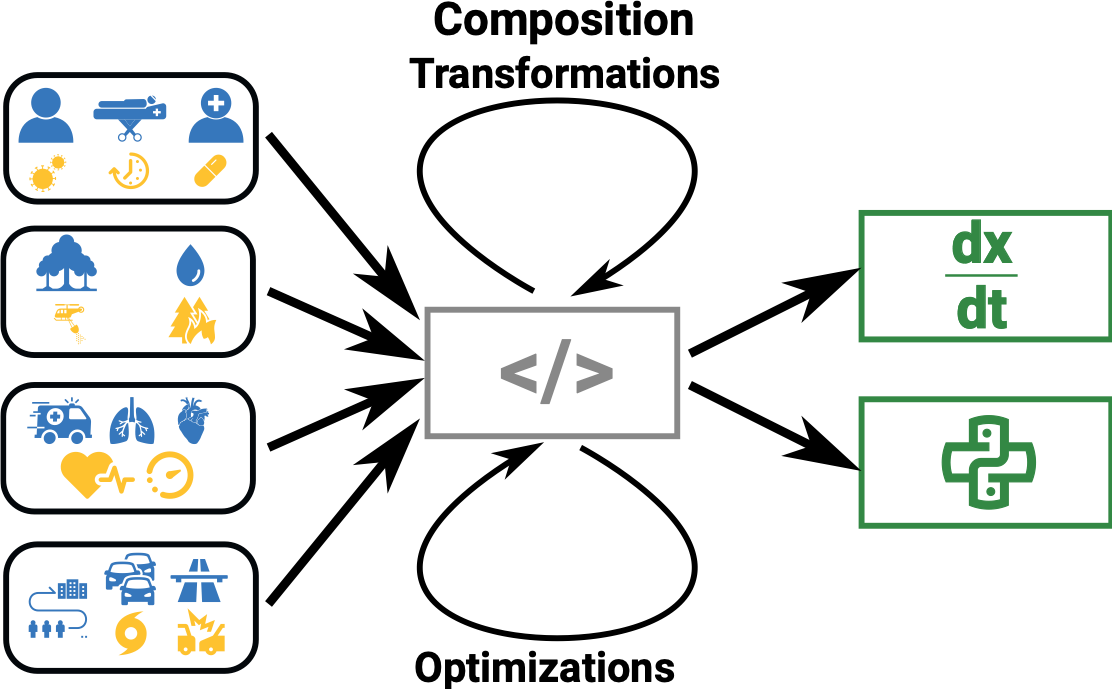
\includegraphics[width=\textwidth]{figs/AMIDOL-flow.png}
  \caption{Decomposing \amidol{} into the metamodeling stack.}
  \label{Fig:AMIDOL-Flow}
\end{figure}

\amidol{} divides naturally into this modeling stack-centric view.
Figure \ref{Fig:AMIDOL-Flow} illustrates this division.  The VDSOLs
provided by \amidol{} attempt to capture the domain knowledge of the
Abstract Knowledge Layer.  The \amidol{} IR translates this
information into the Structured Knowledge Layer.  Finally the
\amidol{} Inference Engine generates executable code from the IR,
forming the Executable Knowledge Layer.

To better formalize this process, and avoid the overuse of the term
``model'' and ``modeling'' in ways which create ambiguity we introduce
several new definitions:

\begin{mydef}[Formulation]
  A formulation is a high-level domain model which represents and
  encodes semantic domain knowledge about a complex system.
  Formulations are the model-stack equivalent of a high level
  language and should focus on being accessible to domain scientists.
  While formal semantics may be implied by a formulation, the primary
  point of formulating a model is not writing down executable code or
  mathematical representations.  It is
  writing down assumptions and knowledge which can, at a later stage,
  be used to infer these properties of a model.

  Formulations should be represented in a form that is close to
  natural language, or natural representations, such as diagrams, used
  by domain scientists.

  Formulations define the Abstract Knowledge Layer of the modeling stack.
 \end{mydef}

 \begin{mydef}[Representation]
   A representation is an intermediate-level model which
   represents the syntactic consequences of domain knowledge about a
   complex system.  While not executable by themself, they express
   information or knowledge about systems in a structure that is
   defined by a consistent set of rules.  These rules can then be 
   reasonabed about to interpret the meaning of components in the
   structure.  At a minimum a representation should explicitly store
   the state of the model in some sort of static semantics on data,
   and provide a set of execution (or dynamic) semantics that provide
   strategies for expression evaluation, or a manner of resolving
   control structures.  This allows for formal and unambigious
   reasoning about how the constructs of a representation result in
   system behavior with respect to state variables.

   Representations define the Structured Knowledge Layer of the
   modeling stack.
\end{mydef}

\begin{mydef}[Implementation]
  An implementation is a low-level, machine and library specific,
  model which serves as executable code, providing the ability to
  perform inference on a complex model.

  Implementations define the Executable Knowledge Layer of the
  modeling stack.
 \end{mydef}

 \subsection{Abstract Knowledge Layer}

 \amidol{} represents the Abstract Knowledge Layer with  formulations
 expressed in a given VDSOL.  These formulations are composed of two
 parts, a directed graph of nouns and verbs, representing high-level
 concepts in the domain along with arcs to express polarity
 relationships; and a reward model on the graph of nouns and verbs
 which ultimately defines an expression on reward variables over the
 graph which define a measure of interest.  These components can be
 thought of as the \textbf{formulation of the system}, and the
 \textbf{formulation of a query} over the system.

 \subsection{Structured Knowledge Layer}

 \amidol{} represents the Structured Knowledge Layer with
 representations expressed in its IR.  These representations are
 expressed in a Turing complete language.  This is an important
 property as it means the \amidol{} IR can represent any computable
 function, and thus, a formulation of any complex system paired with a
 formulation of any computable reward can be translated into
 \amidol{}'s IR.  \amidol{} achieves this Turing completeness by
 leveraging two proofs about Petri nets, from which it inherits much
 of its syntactic properties.

The first important property stems from the three main categories of
Petri nets defined in the literature \cite{reisig2012petri}:
\begin{itemize}
\item Condition-event nets (C/E-nets).
\item Place-transition nets (P/T-nets).
\item Predicate-event nets (P/E-nets).
\end{itemize}

C/E-nets have a restriction that constraints each place in the net to
either a value of 0 or 1, i.e. a place may contain one ``token'', or
no tokens.  This means an event in a C/E-net may not change the value
of a down-stream place as a result of firing, if that place already
has a value of 1.  To be classed as a P/T-net the Petri net must lift
the restriction of a single token residing in a given place present
for C/E-nets.  While this opens the door to infinite state-spaces, it
also gives a petri-net the equivalent of an infinite bi-directional
tape required for Turing machines \cite{reisig2012petri}.

The second property exploited by \amidol{}'s IR for Turing
completeness is the implementation of appropriate logic through its
predicates to be equivalent to a One Instruction Set Computer (OISC).
It has been shown that the full control logic of a Universal Turing
Machine can be implemented with a single instruction
\cite{mavaddat1988urisc}.  Such instructions require the ability to
perform negation, or inhibition of a path of control flow.  Petri nets
commonly enable this through the use of inhibitor arcs
\cite{ciardo1994petri} and P/T-nets with inhibitor arcs have been
shown capable of implementing a Universal Turing Machine
\cite{hack1976petri}.

\amidol{}'s IR avoids a simple Petri-net representation, however, for
reasons which are analogous to the reasons why chip manufacturers do
not, in practice, implement performable computers as OISCs.  Because
some guard conditions on control logic can provide exponential
explosions in the number of arcs and places needed to represent a
given Petri-net \cite{sanders1991reduced} \amidol{} uses boolean
predicates on the inputs and outputs to compactly represent control
flow and avoid this exponential explosion in the IR, which would make
it impractical to use for some models.

\amidol{} encodes all representations in its IR.  Any optimizations,
compositions, or translations on the IR result on a new representation
which is also in the IR.  Because of the Turing Completeness of the
\amidol{} IR, it provides an ideal core for the \amidol{} stack which
abstracts away both the details of the executable target, and the
domain formulation.  This also means that applicable results from
one domain (perhaps predictions on viral reproduction rates
derived from a stochastic chemical model) can be applied to other
domains which utilize different formulations (such as predictions of
infection rates in organisms) easily, since both have representations
in the same IR.

\subsection{Executable Knowledge Layer}

\amidol{}'s Executable Knowledge Layer consists of an application
which compiles the \amidol{} IR into executable code, linked to
appropriate libraries, which solves the reward structures defined by
its IR in a way which can be translated into a solution to the
originally formulated query.  By examining the properties of a given
IR \amidol{}'s Executable Knowledge Layer is able to determine what
libraries are appropriate for solution.  For example, even though a
model in the IR might be representable as a system of differnetial
equations, if the \amidol{} inference engine determines that the
state-dependent rates of a given model may result in a stiff system of
differential equations, it will be able to note that traditional
solution is not a performable option, and either represent the system in an
alternative manner (if the state space is finite, successive matrix
multiplication, for example), or alert the user to non-performable
behavior which may indicate errors.

Results from this layer is then stored in a database, for eventual
translation back up the modeling stack.

\section{Roadmap for \amidol{} and Collaboration}

\begin{figure}
  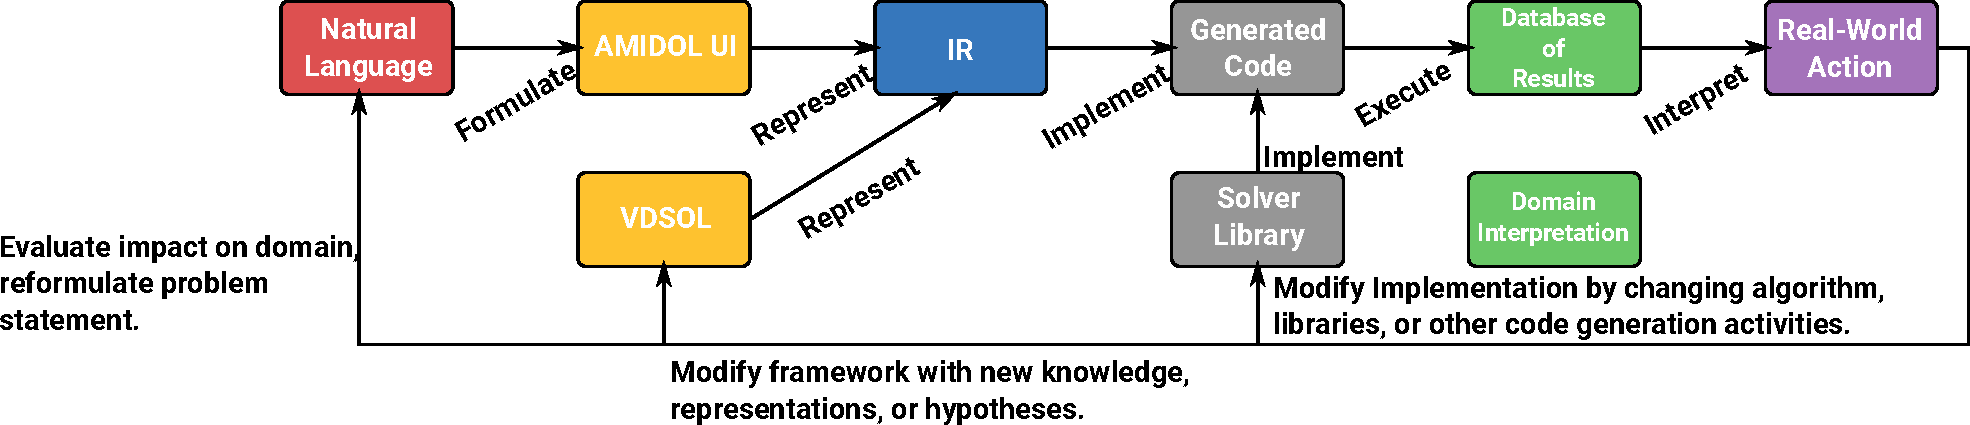
\includegraphics[width=\textwidth]{figs/meta-model-diagram-AMIDOL.pdf}
  \caption{An operational view of the \amidol{} implementation of the
    ASKE Modeling Stack.}
  \label{Fig:AMIDOL-Ops}
\end{figure}

Key challenges for Phase II of \amidol{} involve finalizing the
current specifications of \textbf{forumulations},
\textbf{representations}, and storage of results of the execution of
\textbf{implementations} for later transfer up the stack, and making
these specifications and their current implementations available to
other performers.  Figure \ref{Fig:AMIDOL-Ops} shows the current plan
for \amidol{}'s final operational diagram, and end-to-end process for
machine-assisted modeling, and machine-assisted inference on
formulations.

During Phase II, we will implement additional VDSOLs, in adjacent
domains, to help demonstrate the transfer of knowledge across domain
formulations to show the potential provided by the ASKE Modeling Stack
approach to machine-assisted inference.  In addition we will work with
our collaborators at GTRI and the University of Arizona to ensure the
interoperability of our implementations at the Structured Knowledge
Level, to help demonstrate the power provided by a Turing Complete
representation, and the ability to propagate models up the stack
resulting in new abstractions, and knowledge extraction at the
formulation level, such as discovering model equivalences.

We are making plans already for a collaborative visit to GTRI in
mid-June, and hosting weekly collaborative meetings over Google
Hangouts to begin defining mechanisms to interoperate with our
colleagues, and defining additional solver targets we can provide for
our backend to illustrate efficient analysis of the executable needs
of implementations of a given representation; as well as targets which
will be relevant and useful to our collaborators at GTRI and the
University of Arizona.

As a mid-Phase goal, we plan to demo our combined system in September
a the World Modelers' demo day, if space and time can be allocated by
the organizer.

\section{Resources, web sites, etc.}

The current \amidol{} source code, including example models and documentation, is available at the \amidol{} Github site \url{https://github.com/GaloisInc/AMIDOL}.

\bibliography{AMIDOL-MWS}

\end{document}
